\chapter{Reports and Facilities Management}
\label{sec:rm}

The use-case for Taarifa tightly couples the reports management and facilities management. However, as this project may be used solely for reports management, or solely for facilities management, or as a reports-cinema manager, the implementation of reports management is not coupled to facilities. \\

The reports management has been designed as an interface which can be implemented by apps, to make models reportable. \\

Currently only a programmer is able to make reportable models, but future versions of the software could enable this to be done through the admin interface. \\

The facilities management without the reports management is one model which is registered with a slightly customised ModelAdmin. \\

As such, there is little to say about the facilities management without the reports, so the two are discussed together in this chapter.

\begin{figure}
\centering
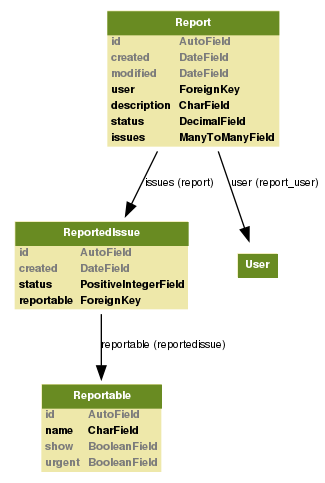
\includegraphics[scale=0.51]{img/reports.png}
\caption{Figure to show UML diagram for the reports management}
\label{fig:rm:uml}
\end{figure}

\FloatBarrier
\section{Reports Interface}
The interface defines two abstract classes and one abstract form class. The UML diagram for the abstract classes is shown in Figure~\ref{fig:rm:uml}; and the class diagram for the form is shown in Figure~\ref{fig:rm:forms}.

To declare an app as reportable, it must have at least two models, one of which subclasses ReportedIssue, and the other Reportable. In order for a user to create a report, the app must contain a form which subclasses ReportForm. A view which contains this form can be presented to the user. On submission of this form, reports are automatically created. All reports created are automatically displayed on the admin page. \\

The form's default behaviour is to present all Reportables in the system as a list of checkboxes for the user to tick.

\subsection{Reportable}
The Reportable class is an abstract representation for an item in the system which can be reported. For example, a toilet. \\

As many subclasses of Reportable can be declared as a programmer desires.

\paragraph{Show} is a boolean to determine whether or not an instance should appear on report forms. When a model instance is deleted through the Django admin, all foreign key relations are also deleted. If a Reportable were able to be deleted, user submitted data would be deleted too. To prevent this from happening, an administrator cannot delete a Reportable once it has been created, they can only toggle its display with this checkbox.

\paragraph{Urgent} A boolean which an administrator can use to indicate if a report on the Reportable should be flagged as urgent. This is used by the auctions app.

\subsection{ReportedIssue}
A Reportable can be reported many times by different users, but once it is flagged as such, this need only be in the database once. A ReportedIssue is created the first time a report is made for the Reportable. \\

Only one ReportedIssue can be handled by the report form. No use-case could be conceived where more than one would be required.

\paragraph{status} The values in this field are discussed in more detail in Appendix~\ref{app:statuses}. When the status of a ReportedIssue is changed, the user is notified of the change. They can currently toggle notification for all status changes, but in the future they will be able to do this on a per ReportedIssue basis. \\

Once the status is set to ``Fixed", a ReportedIssue will be created the next time that Reportable is reported.

\subsection{Report}
This class is not designed to be subclassed. One instance is created every time a report form is submitted, storing data of the user who made the report and all the Reportables reported.

\paragraph{status} is the percentage of the completed ReportedIssues. This could be calculated on a per-request basis to save the extra work which recalculates the value when the status of a ReportedIssue changes. It was decided that a user might check the status more often than it changes, so calculating the value and storing it may slightly improve efficiency. Otherwise, each time a user wishes to know the status of a report, the Many-to-Many issues field would have to be traversed.

\paragraph{description} Any additional information the user wishes to add.

\subsection{ReportForm}
\label{sec:rm:reportform}

\begin{figure}
\centering
\includegraphics{uml/reports-forms.1}
\caption{Interface diagram for reports management forms}
\label{fig:rm:forms}
\end{figure}

\begin{figure}
\centering
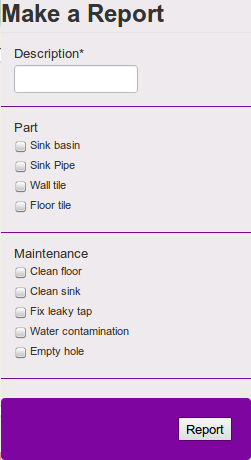
\includegraphics[scale=0.4]{img/reportform.png}
\caption{Example of an implemented ReportForm}
\label{fig:rm:reportform}
\end{figure}

For an app to display a ReportForm which automatically generates the checkboxes of Reportables specific to that report, it can subclass this form.

\paragraph{action} is the form action: the URL to which the form is posted.

\paragraph{reportables} is a list of all Reportables to be displayed as checkboxes on the form. This defaults to the immediate subclasses of Reportable. Every instance of the model will be rendered as one checkbox, under the title of the Reportable. In Figure~\ref{fig:rm:reportform}, the Reportables are ``Part" and ``Maintenance", and the instances are the checkboxes.

\paragraph{reported\_issue} is the subclass of ReportedIssue which has been implemented.

\paragraph{extra\_reportable\_args} are extra arguments which can be provided to the query which retrieves Reportables from the database.

\paragraph{get\_extra\_create\_args} If this method is not implemented, a NotImplementedError is raised. When a report has is being saved, a database call is made to see if there are existing ReportedIssues for a given Reportable. A Reportable may be associated with more than one object. For example, 450 facilities have one Reportable toilet. There only need be one toilet which the 450 facilities point to. Therefore, the id of the Reportable is not enough to check the database for existing ReportedIssues, and additional arguments must be provided. The function is given the Reportable currently being saved.

\paragraph{clean\_reportable} is an optional function which is called when ReportForm is being validated. It is passed the class of the Reportable being validated, and a list of all checkboxes. This could be used, for example, to prevent two Reportable instances from being reported together.

\section{Facilities Management}
The facilities management implements the interface discussed in the previous section to allow facilities to be reported. The table of user requirements is shown in Table~\ref{tab:rm:fac:req} and the UML for the app is in Figure~\ref{fig:rm:fac:uml}.

\begin{figure}[thp]
\centering
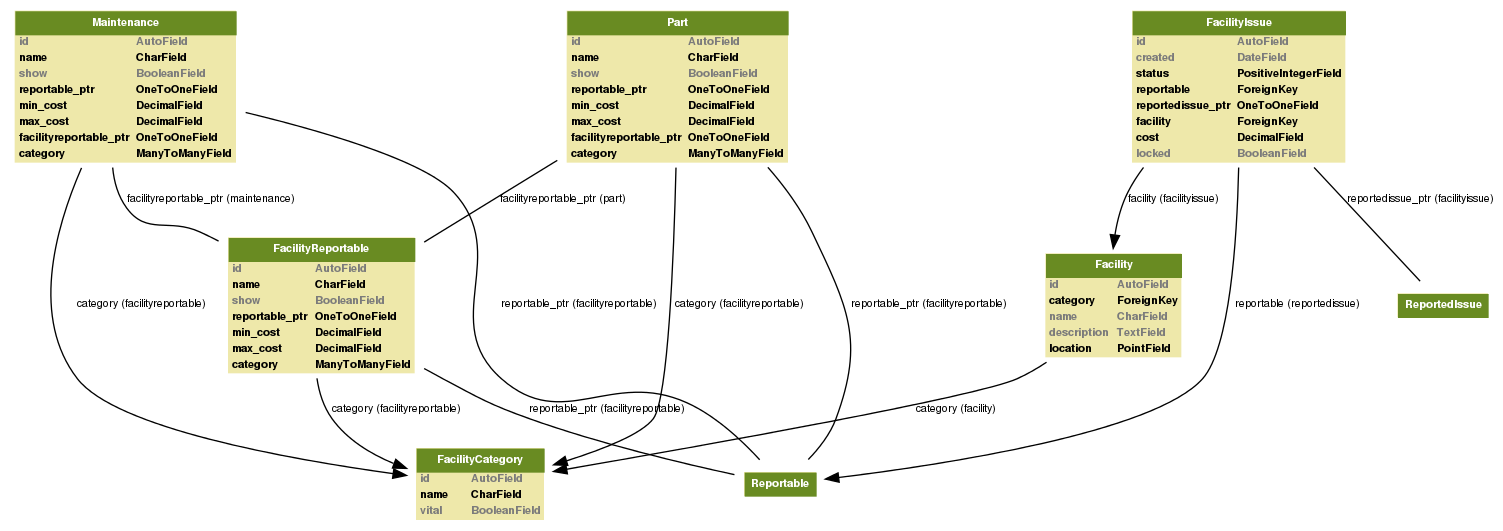
\includegraphics[scale=0.35,angle=90]{img/facilities.png}
\caption{UML diagram for the facilities management}
\label{fig:rm:fac:uml}
\end{figure}

\subsection{User Requirements}
\begin{table}[h]
\centering
\begin{tabular}{p{2.9cm}p{4.1cm}p{4.1cm}}
\textbf{As a...} & \textbf{I want to...} & \textbf{because...} \\
\hline
Administrator & Add, change and delete facilities & I want full control over the facilities \\
\hline
Administrator & Add, change and delete parts for each facility & I want to specify a parts list \\
\hline
Administrator & Add, change and delete services for each facility & Some problems are not parts, and they require service. \\
\hline
Administrator & View reports made on each facility & I want to keep an eye on citizen happiness \\
\hline
Administrator & Change the status of issues & I want to control the system \\
\hline
Citizen & Report a facility problem on my phone or with a website & I'm unsatisfied with something in my town \\
\hline
Citizen & See the status of the reports I have made & Be updated on the happenings of the town \\
\hline
Citizen & Provide feedback on how the report was handled & I believe in customer service \\
\hline
Citizen & See a map of reports in my area & Someone may have already reported the problem I care about \\
\end{tabular}
\caption{Table to show user requirements for the facilities management system}
\label{tab:rm:fac:req}
\end{table}

\subsection{Facility}
The data in Taarifa was exported from \gls{OSM}~\cite{openstreetmap}, who are currently collating geographical data in Africa~\cite{openstreetmapafrica}. As such, it was decided to model the Facility class on the data exported from \gls{OSM}. \\

\paragraph{location} is a GeoDjango PointField, which enables geo-spatial queries to be performed on the facilities.

\subsection{FacilityCategory} Every Facility is categorised, and in Taarifa, this is either ``toilets" or ``drinking\_water" (taken directly from \gls{OSM}). \\

\paragraph{Vital} was added when it was decided the urgency of reports could not be handled automatically. If a report is made which is not marked urgent, but does come from a Facility which is vital, it will be moved through the auctions system more quickly. \\

\subsection{FacilityReportable}
This is the class which subclasses Reportable. For facilities management, it was decided to have a Parts list and a Maintenance list. \\

The Parts list is a way for an administrator to keep stock of the Parts in the facility. In the future, this could be connected to local businesses for stock-ordering. \\

A Maintenance list is a list of maintenances which may need to be performed. Part and Maintenance are identical classes and are both Reportable. As such, they inherit from FacilityReportable which is abstract.

\paragraph{cost} is the estimated cost to service a broken part or to perform a maintenance.

It was decided that Facilities of the same FacilityCategory would have the same parts, give or take one or two. This is why FacilityReportables has a relationship to FacilityCategory and not Facility.

\subsection{FacilityIssue}
FacilityIssue subclasses ReportedIssue.

\paragraph{cost} is automatically filled in with the cost of the FacilityReportable when an issue is created (by implementing get\_extra\_create\_args). However, an administrator may decide that they wish to overwrite this field when the issue is reported.

\paragraph{locked} is to prevent a read-update race condition happening when updating the cost. This field is specifically implemented for use by the auctions app.

\subsection{Facility ReportForm}
This was an implementation of the ReportForm. As an example of how straightforward it is, the entire class is 16 lines of code.

\subsection{Implementation}
\subsubsection{Admin}
A script has been written to read data in an \gls{OSM} .osm file and convert it into Facility objects. Currently this is not available through the admin interface, but will be implemented in future. This allows for bulk imports of Facility data. \\

When adding a facility, the system checks to see if it's within the bounds defined in the config file. If not, the facility cannot be saved. Originally these bounds were also displayed, but it looked bad and was tricky to implement without breaking. It is assumed that the administrator knows the bounds of his own site. For multiple sites using the same database, the ``current site" will have to be toggled to add facilities. This is not a use-case anticipated to happen often. \\

All reports made can be viewed through the administration section. The reports are read-only. \\

Facility is registered through the admin, and django-olwidget~\cite{olwidget} is used to present the facilities on a map. An administrator can click the facilities and be taken to the editing page. Facilities cannot be deleted through the interface because this would delete past data. \\

The administrator has full control over the Parts and Maintenances, apart from deleting. \\

An administrator can view all the currently open reported issues with the facility. If the boolean for locked is not set, they are able to change the price of the issue. If the lock is on, an auction is in place and they can no longer do this. \\

The administrator can only change the status of a job from ``Dispute Resolution" to ``Complete". This is because the jobs system handles the issues' status automatically.

\subsubsection{Citizen}
When the status of a report changes, the citizen is automatically sent an SMS. \\

The vision for a user in Tandale using this system is they will be sat on the loo, or squatting over the hole, and a pipe will burst. They will pull out their phone, go to the website and report a problem straight away. They do not want to register or login. \\

The mobile version of the site uses HTML5 browser geolocation to determine where the user currently is. This is automatically sent to the server, which retrieves the report form for the nearest facility to that location. Therefore, the first thing a mobile user will see is a report form. \\

To submit this form, they do not need to register: an account will automatically be created for them and verification sent to their mobile phone. \\

The website version's homepage is a large map with clickable facilities. When clicked, a report form tailored to that facility appears (Figure~\ref{fig:rm:fac:home}). To submit the form, a user must register manually with their mobile phone, and return the verification code. A worker nor an administrator has the option to report a problem. Workers cannot report problems to prevent them from false reporting to get jobs.

\begin{figure}
\centering
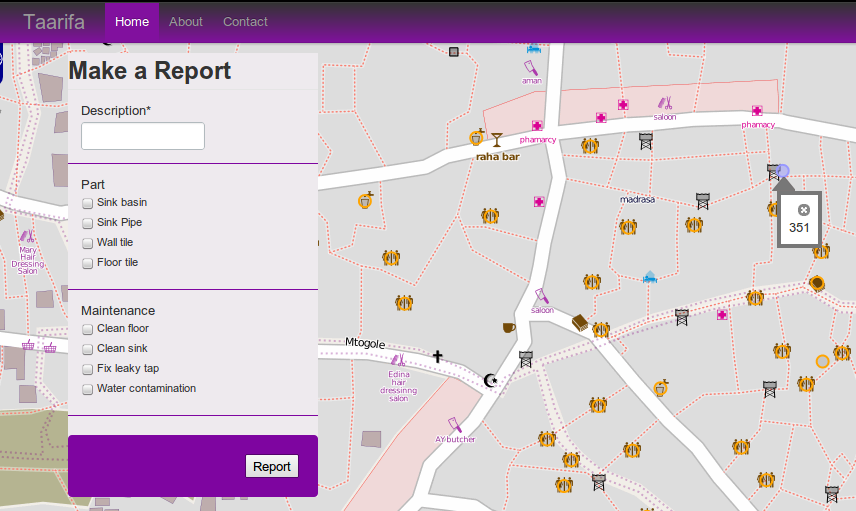
\includegraphics[scale=0.4]{img/home.png}
\caption{Truncated view of the home page}
\label{fig:rm:fac:home}
\end{figure}

\FloatBarrier
\section{Performance}
\label{sec:rm:fac:perf}

There are Many-To-Many relations defined throughout the classes, and these may cause performance issues. The bottleneck when creating a report would occur when the system is checking for existing ReportedIssues. \\

A script was written to generate a report, and then delete the report 10,000 times, and the total time recorded for each creation, and then averaged. \\

Originally, this was run with each issue created treated as a separate database call. The average time taken to create a report was 0.3182691201s. \\

Wrapping the script in a transaction decorator, which sends a transaction to the database, this time was reduced to 0.1430310377s on average. \\

The same process was repeated without deleting the reports, so 10,000 reports were added to the system. The time taken was 0.1488591671. \\

Therefore, there is no bottleneck when there are many reports in the system.